\chapter{Clustering algorithms in high energy physics}
\label{ch:1}
\section{The clustering problem}
\label{ch:clustering_problem}
Cluster analysis is, in general, a non trivial problem. Even the definition of cluster can change wildly depending on the context. Due to these circumstances many clustering methods have been developed, based on various notions of cluster\cite{clustering}. Currently, some of the most common clustering algorithms can be divided in the following categories: 
\begin{itemize}
    \item Connectivity models: generally based on distance between points;
    \item Partitioning: such as k-mean algorithms, represent each cluster by optimizing a single function which depends on the distance\cite{k-mean};
    \item Density models: consider dense regions in the data space as clusters;
    \item Hierarchical methods: build clusters following a recurring dendrogram with splitting or merging.
\end{itemize}
There is no general correct way to produce clusters: each problem requires a specific approach depending on the conditions known a priori, the expected results and also the desired performance. This is why it was necessary to develop a specific algorithm to cluster hits in CMS's calorimeters.

In the upgrade plan for the future revision of LHC, HL-LHC (High Luminosity Large Hadron Collider), calorimeters with high readout granularity have been suggested to observe fine grained images of hadronic and electromagnetic showers\cite{high_granularity}. In the case of CMS, the planned endcap calorimeter (HGCAL) will be based on hexagonal silicon sensors with a surface area of 0.5 or 1 cm$^2$\cite{hgcal}. Following a collision, when a particle showers, the resulting energy is collected by the sensors on the layers that the shower goes through. By clustering the resulting energy deposits (hits) it is possible to reconstruct the shower dynamics and identify all of the hits caused by a single particle. Since the calorimeter will have a high granularity, the most efficient way to cluster the deposits is to group them in bidimensional clusters layer per layer\cite{2d} and then relate the clusters in different layers. In this context, a computational challenge arises, due to the large amount of data and the limited computational time available. Since event reconstruction must happen at millisecond-level time frames, the algorithm employed will have to be highly efficient and scale well, meaning linearly, as the number of hits increases as not to bottleneck the performance of the event reconstruction. These specific requirements have brought CMS to explore the potential of heterogeneous computing with hardware accelerators such as GPUs or FPGAs which can take on part of the work achieving a higher throughput and better energy efficiency. 

In any case, the input to any clustering algorithm is a set of $n$ hits and the output is a set of $k$ clusters which is usually one or two orders of magnitude smaller than n. For clustering in high energy physics, n usually varies from a few thousands to a few millions, while k generally depends on the number of incoming particles as well as the number of layers of the calorimeter. For CMS HGCAL, we can estimate the average number of hits in a cluster $m=n/k$ to be in the order of 10. This leads to the relation between the number of hits $n$, the number of clusters k and the average number of hits in a cluster $m$ as $n > k \gg m$. Let's analyse some of the possible clustering methods cited above. Starting from partitioning algorithms, these are not applicable in our case since the number of clusters $k$ is not known a priori. Moving to hierarchical clustering, this method is not suitable as well, since it does not scale well as each decision to split or merge needs to scan over many objects or clusters. Density based methods are the most interesting for our application, as they are capable of discovering clusters of any shape and are efficient for large spacial database. However, well-known existing density-based clustering algorithms intrinsically include serial processes that are hard to parallelize. With all of this in mind, CMS developed a clustering algorithm of its own.

\section{CLUE standalone}
\subsection{What is CLUE?}
\label{ch:clue}
Clustering of Energy (CLUE) is "A fast parallel clustering algorithm for high granularity calorimeters in high-energy physics"\cite{CLUE} it was specifically developed to address all of the aforementioned challenges in clustering hits in high granularity calorimeters. This algorithm follows a density-based approach with some specific optimizations implemented to allow for a greater expression of parallelism. Starting from the beginning, the input data for the algorithm is a series of hits each with its corresponding coordinates (x, y and layer) and energy. For each point, two key variables are calculated: the local density $\rho$ and the separation $\delta$. The first one represents the energy density in the area of the hit, while the second variable corresponds to the distance from the hit and the nearest hit with higher local density. From these two parameters it is possible to cluster points depending on arbitrary thresholds imposed on a case-by-case basis. 

\subsection{Clustering procedure}
\label{ch:clustering_procedure}
Since CLUE was specifically designed to be used in high-energy calorimetry, where hits are registered on sensor cells whose layout is a multi-layer tassellation, the algorithm's data is indexed with a fixed grid, which divides the space into rectangular bins. This indexing choice allows to query information for multiple points at the same time to better express parallelism on GPUs and when running on multiple threads.

CLUE requires three parameters: the critical distance, $d_c$, is the cut-off distance in the calculation of the local density, the critical density, $\rho_c$, is the minimum local density to promote a point as a seed or the maximum density to demote it as outlier, finally the outlier delta factor, $odf$, is a multiplicative constant applied to the critical distance and defines the maximum distance between a point and its nearest point with higher density to promote the point as a follower. These parameters are chosen at run-time and can be tuned by the user to be based on the specific physics of the events that they are clustering. For example, $d_c$ can be tied to the expected shower size and the granularity of the detectors (possibly differing between silicon-based layers and scintillators), $\rho_c$ can be tuned to maximize the signal to noise ratio and $odf$ can be chosen considering the showers separations. In this way, the use of configurable parameters allows CLUE to be more flexible at clustering different events for the specific desired goals of physics. 

\begin{figure}[ht]
    \centering
    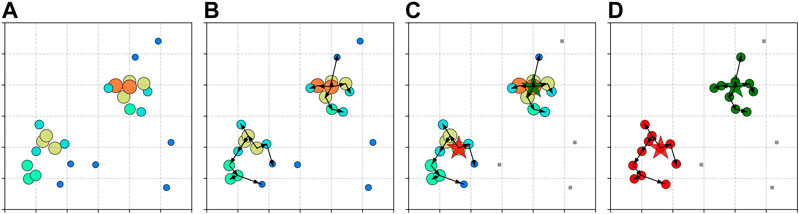
\includegraphics[width=0.9\textwidth]{media/clustering_procedure.jpg}
    \caption{Schematic representation of CLUE clustering procedure: from fixed spacial grid to clusters.}
    \source{\emph{:} \cite{CLUE}, figure 2}
    \label{fig:clustering_procedure}
\end{figure}

In figure \ref{fig:clustering_procedure} the clustering procedure of CLUE is exemplified in a $6\times6$ grid. First, a fixed grid is constructed, then CLUE calculates the local density $\rho$ of every point in the discrete space created by the grid as shown by the different sized and colored dots (A). Then, each point gets assigned a nearest higher $nh$, that is the nearest point with higher local density (B). The distance, $\delta$ from this point is one of the deciding factors to promote to seed or demote to outlier. Now, points with $\rho$ higher than the critical density $\rho_c$ and separation greater than the product of the critical distance $d_c$ and $odf$ get promoted as seeds, while points with lower density and large separation ($\delta > d_c \times odf$) get demoted to outliers. Points that are neither seeds nor outliers are followers of some other point, so a list of followers is built for each point considering points with the same nearest higher. In other words, Every seed has a chain of followers which can have followers themselves and this creates a cluster. Clusters are farther away than $d_c \times odf$, meaning that no point from one cluster is closer than that to any point from any other cluster. Outliers are simply points with no followers and are not followers of any other point as well.

\subsection{GPU implementation}
\label{ch:gpu_impl}
As previously discussed, CLUE was first developed in order to provide a parallelizable clustering algorithm for high occupancy scenarios in high energy physics. Let us dive a little deeper in the ways that CLUE's implementation takes advantage of the multi-threading capabilities of GPUs. The main advantage of this class of accelerators is given by their massive number of physical threads each one of which can be used to make computations regarding a single point. Because of this, the GPU implementation of CLUE assigns one GPU thread to each point, for a total of $n$ threads, to create the spacial grid, calculate the local density and separation, promote or demote the point and register points as followers of the corresponding nearest higher. After this, one thread gets assigned to each seed, $k$ threads in total, to expand the clusters along the followers' chain. Since the results of each step are required in the following ones, it is necessary to synchronize all of the threads before moving onto the next computation. This is naturally done by implementing each step in a separate kernel. Data for all of the points is stored in the global device memory as a single structure-of-array (SoA), which contains the points' coordinates, layer numbers and weights. 

One key factor to take into consideration when developing software for GPUs is that, due to the parallel nature of the execution, it can happen that multiple threads try to access and modify the same address in global memory at the same time. In particular, in CLUE thread conflicts can happen in three cases:
\begin{enumerate}
    \item multiple points need to register to the same bin simultaneously;
    \item multiple points need to register to the list of seeds simultaneously;
    \item multiple points need to register as followers to the same point simultaneously.
\end{enumerate}
Because of this, some atomic operations are required to avoid race condition among threads. During one of suck operations a thread is granted exclusive access to a specific memory location that becomes inaccessible to all other threads until the atomic operations finishes. The usage of atomic operations naturally causes some serialization among threads in a race. Its impact is negligible in cases 1 and 3, since the bin dimension and the number of followers per point are usually small. By contrast, serialization in case 2 can cause significant slowdowns since the number of seeds $k$ can be large. However, the atomic pushing back to the list of seed is still faster on GPU memory compared to the data movement between host and device, so the total execution time of CLUE does not suffer significantly from this serialization.

\section{Framework integration}
\label{ch:framework_integration}

\subsection{The need for heterogeneous computing}
\label{ch:heterogeneous}
The high luminosity upgrade for the LHC, scheduled before the beginning of the next runs from 2029 onwards , will increase the number of collisions per second (luminosity) by roughly a factor of 10 with an average pileup of 200 proton-proton collisions. Such an increase in the number of events per second will pose an incredible challenge for both online and offline reconstruction software built by the experiments \cite{high_luminosity}. This added complexity far exceeds the expected increase in processing power for conventional CPUs and thus calls for different solutions. One such possibility is $heterogeneous computing$ which is already being exploited by industry and high performance computing centers to achieve better efficiency and higher throughput by matching the job to the best possible architecture. Specifically, applying this new paradigm to CMS's reconstruction software (CMSSW) and its framework means that part of the work can be offloaded to one or more graphics processing units (GPUs), thus easing the load on the CPU while simultaneously increasing the total throughput and improving energy efficiency. Tasks offloaded to GPUs can and will be executed in a parallel fashion and, most importantly, in an asynchronous manner with respect to code running on the CPU, meaning that the host resources freed by offloading work to GPUs can be used for other tasks at the same time. The shift to heterogeneous computing has already proved to be a success for CMS offline reconstruction with GPU implementations showing as much as a three time increase in performance in some cases \cite{high_luminosity}. However, shifting to heterogeneous computing also poses some challenges, especially in code portability and maintainability. While having the possibility to offload work on different hardware surely looks promising, it also means that in order to be able to efficiently execute software on heterogeneous hardware, the code should be written and optimized for each specific back-end\footnote{In software engineering, the physical infrastructure or hardware on which the code is executed.} to be targeted. Even considering only mainstream GPU manufacturers, one would need to take into account three different implementations for each and every kernel in all of the algorithms. Moreover, maintaining such a massive amount of code would represent an insurmountable challenge and a great resource sink. 

These reasons are what led to look for an appropriate compatibility layer to ease the transition to heterogeneous computing. Such a layer would have to support multiple architectures letting the programmer write a single source code without having to sacrifice performance. 

\subsection{SYCL and others compatibility layers}
As previously discussed, the shift to heterogeneous computing, while improving performance and efficiency, also poses a great challenge in the ability to maintain code and port it to different architectures should the need arise: this is where portability layers come into play. Especially in recent years, development on these layers has ramped up significantly as more and more applications require to offload work to different accelerators. Many different solutions are now available, with each proposing a different way to tackle the problem, while all trying to use a single source code to produce a unique executable able to run on as many different back-ends as possible. In this context, the CMS collaboration and in particular the high level trigger (HLT) developers have started looking for a suitable compatibility layer to use to write heterogeneous event reconstruction code. The wider CMS reconstruction software (CMSSW) has successfully been ported to CUDA a few years ago so it is already being executed in a mixed fashion: part of the work is being done by CPUs while other parts, computationally more expensive, are offloaded to NVIDIA GPUs. This is why a great part of the framework has already been ported to such a compatibility layer and this new version is scheduled to go into production after the LHC Christmas shutdown between 2022 and 2023. The compatibility layer currently in use is alpaka: a header-only abstraction library for accelerator development \cite{alpaka}. While we are not going to explore alpaka in detail, it allows the abstraction of the underling levels of parallelism by mapping some custom-defined classes to different hardware depending on the back-end. In general, the work division is very similar to CUDA's grid-blocks-threads division with an extra element added to allow for different mappings on CPUs and GPUs. In this way, the compatibility layer is able to exploit the different parallelization capabilities of each different back-end. As previously stated, reconstruction software has largely already been ported to alpaka which allows to only develop and maintain one source code while still being able to run the reconstruction on both CPUs and NVIDIA GPUs. Support for other back-ends is still ongoing: Intel GPUs are not yet supported by alpaka itself, while AMD GPUs are officially supported, but their back-end has not been implemented in the reconstruction software yet.

Although some other compatibility layers, like kokkos, have been explored, alpaka is, as of now, the most promising of such layers for CMS reconstruction. So, why is SYCL being experimented with? We can propose a few basic reasons for this:
\begin{itemize}
    \item SYCL is an open source project, but is also backed by some big names in the tech industry (such as Intel), which bodes well for the future support of the standard;
    \item As a new compatibility layer is developed, it is always relevant to explore its performance in comparison to native code and other compatibility layers;
    \item While not all back-ends have been implemented yet, SYCL promises to support a variety of devices: from CPUs to GPUs and also Intel's FPGAs.
\end{itemize}
Moreover, being an open source project, SYCL can count on a variety of implementations which we'll explore in a bit more detail in section \ref{ch:sycl_implementations} but at a base level this allows, in principle, for more flexible adaptations of the standard to specific needs. 

% \subsection{An introduction to CMS framework} TODO maybe...